\documentclass[11pt,a4paper]{article}
\usepackage[utf8]{inputenc}
\usepackage[spanish]{babel}
\usepackage{graphicx}
\usepackage{geometry}
\geometry{top=2.5cm, bottom=2.5cm, left=2.5cm, right=2.5cm}
\usepackage{hyperref}
\usepackage{titlesec}

\title{\textbf{Manual de Usuario: Módulo de Contactos y Chatter en Odoo}}
\author{}
\date{}

\begin{document}

\maketitle
\tableofcontents
\newpage

\section{Módulo de Contactos: Organizar y Filtrar Clientes}
El módulo \textbf{Contactos} es la agenda central del negocio. Aquí no solo guardamos datos básicos, sino que también podemos buscarlos de forma inteligente para no perder tiempo.

\subsection{¿Cómo Buscar Clientes rápidamente?}
\begin{enumerate}
    \item En la parte superior derecha de la pantalla de Contactos verás una barra con una pequeña lupa.
    \item Haz clic dentro de esta barra de búsqueda.
    \item Escribe lo que buscas (por ejemplo: el nombre de la empresa, el RUC o el teléfono).
    \item Presiona \textbf{Enter} y la pantalla ocultará temporalmente a los demás clientes, mostrando solo el que escribiste.
\end{enumerate}

\begin{center}
    \makebox[\textwidth][c]{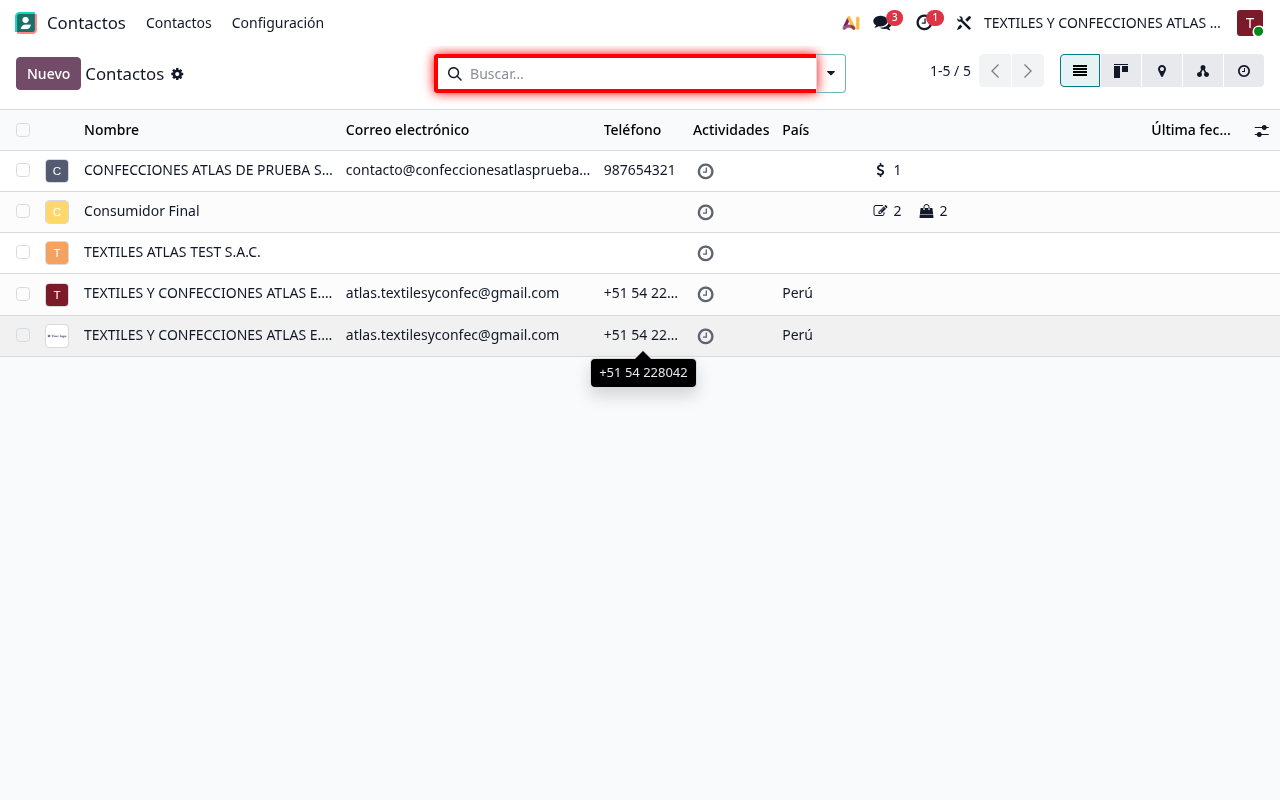
\includegraphics[width=1.15\textwidth]{images/contactos_busqueda_filtros.png}}
\end{center}
\textit{Figura 1.1: Barra de búsqueda superior para encontrar clientes por nombre, RUC o datos de contacto.}

\subsection{Uso de Filtros y Agrupadores (Ordenar a tus clientes)}
Para segmentar a tu cliente rápidamente sin tener que buscar uno por uno:
\begin{enumerate}
    \item Haz clic en el botón \textbf{Filtros} que está justo debajo de la barra de búsqueda.
    \begin{itemize}
        \item \textit{Ejemplo de uso:} Si solo quieres ver a las empresas registradas (personas jurídicas) y ocultar a las personas naturales, selecciona el filtro \textbf{Compañías}.
    \end{itemize}
    \item Haz clic en \textbf{Agrupar por}:
    \begin{itemize}
        \item \textit{Ejemplo de uso:} Si tienes clientes en distintos departamentos del Perú y deseas ordenarlos visualmente por su ubicación, haz clic en \textbf{País/Estado} o \textbf{Ciudad}. Odoo los dividirá de forma ordenada en bloques agrupados.
    \end{itemize}
\end{enumerate}

\subsection{Cambiar de Vistas (Tarjetas vs. Tablas)}
En la parte superior derecha verás tres pequeños botones para cambiar la forma en que se muestra la información:
\begin{itemize}
    \item \textbf{Vista Kanban (Tarjetas):} Muestra cada cliente en un recuadro con su foto y datos rápidos.
    \item \textbf{Vista Lista (Tabla):} Muestra a los clientes en una tabla compacta como una hoja de Excel. Es la mejor opción para comparar datos.
    \item \textbf{Vista Mapa:} Muestra la ubicación geográfica del cliente en Google Maps.
\end{itemize}

\begin{center}
    \makebox[\textwidth][c]{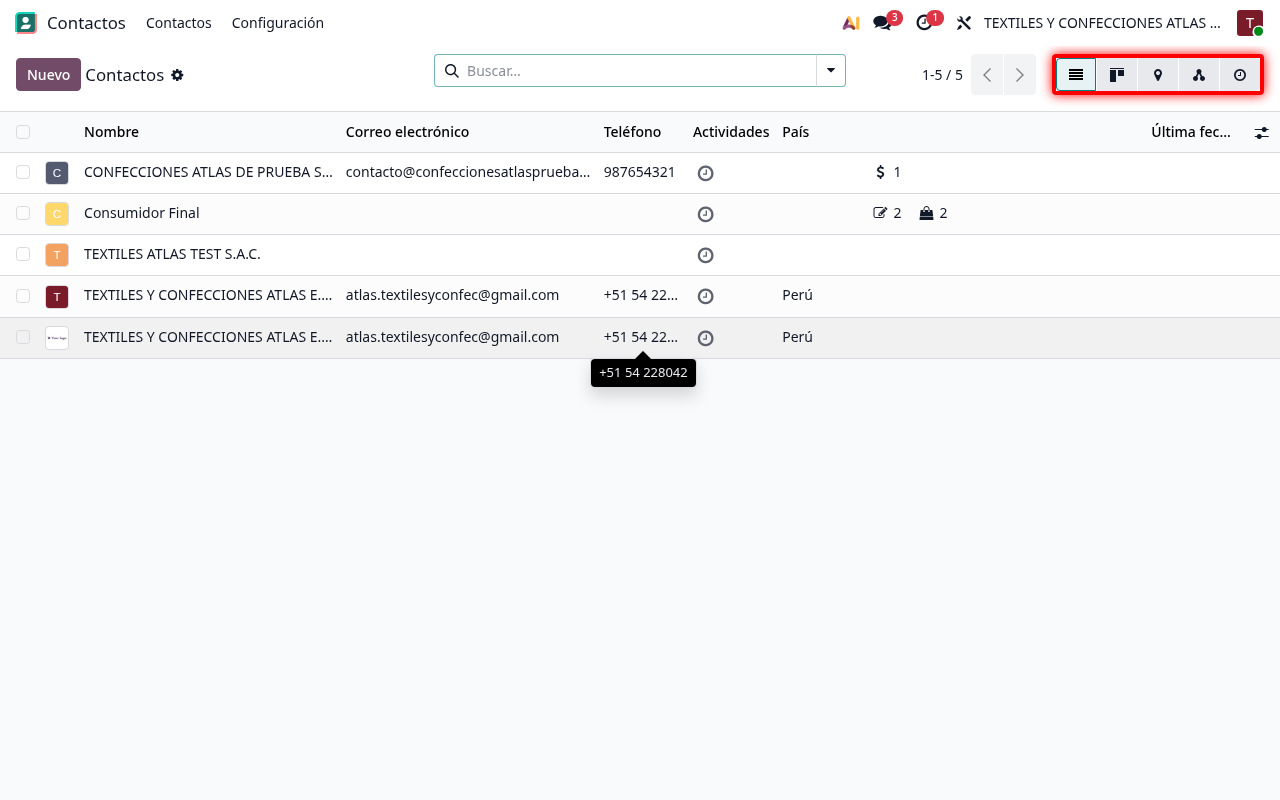
\includegraphics[width=1.15\textwidth]{images/contactos_cambio_vistas.png}}
\end{center}
\textit{Figura 1.2: Botones para alternar entre las vistas Kanban y Lista en Odoo.}
\newpage

\section{El Chatter: El Historial y Centro de Mensajería de Odoo}
El \textbf{Chatter} (sección de comunicación) es una de las herramientas más importantes de Odoo. Se encuentra en el lateral derecho de \textbf{todas las fichas} de Odoo (Contactos, Ventas, Inventario, etc.).

Sirve como una bitácora o cuaderno de notas donde se registra todo lo que pasa con ese cliente para que cualquier trabajador del negocio esté enterado.

\begin{center}
    \makebox[\textwidth][c]{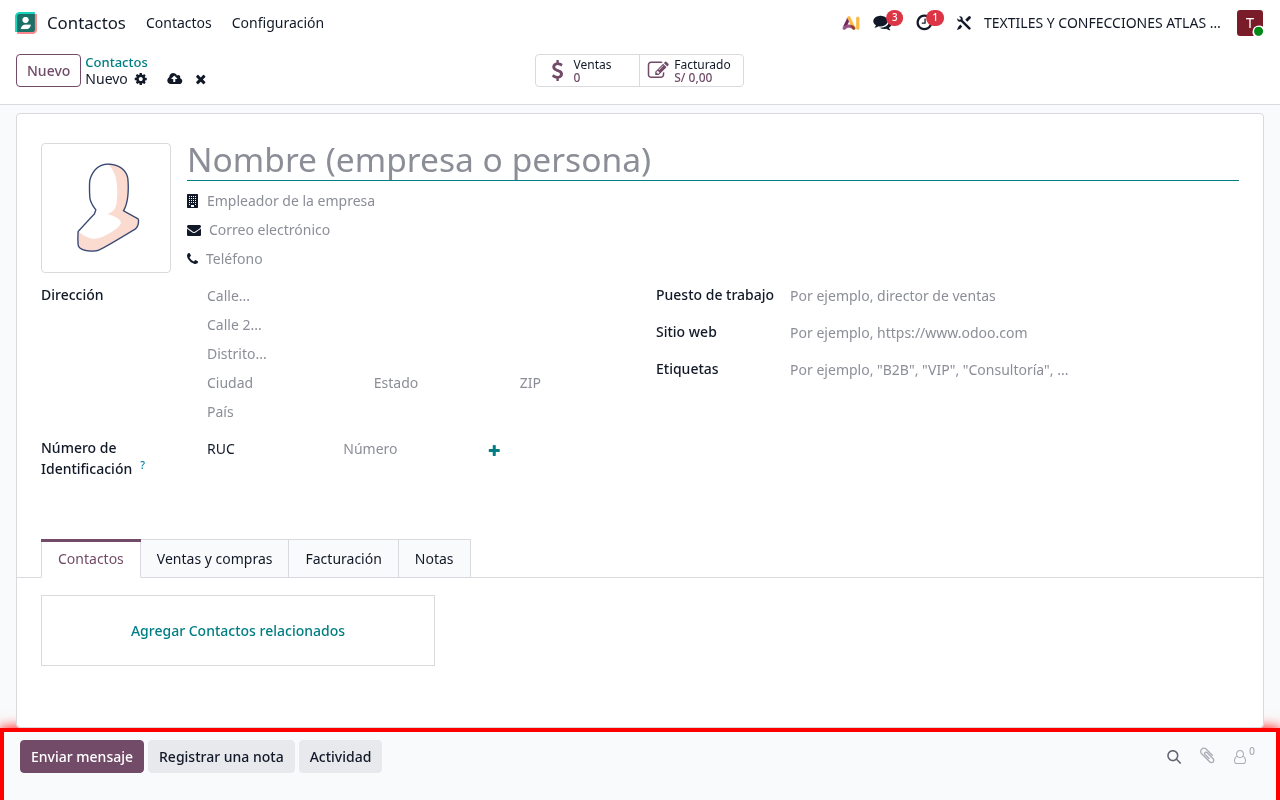
\includegraphics[width=1.15\textwidth]{images/contactos_chatter.png}}
\end{center}
\textit{Figura 2.1: Panel del Chatter en el costado derecho de la ficha del contacto.}

\subsection{Enviar Mensaje (Comunicación Directa)}
\begin{itemize}
    \item \textbf{¿Para qué sirve?:} Para enviar correos electrónicos al cliente directamente desde Odoo.
    \item \textbf{¿Cómo se hace?:}
    \begin{enumerate}
        \item Haz clic en \textbf{Enviar mensaje}.
        \item Escribe tu texto.
        \item Haz clic en \textbf{Enviar}. El cliente recibirá el correo y si responde, su respuesta aparecerá aquí mismo.
    \end{enumerate}
\end{itemize}

\subsection{Poner Nota (Bitácora Interna)}
\begin{itemize}
    \item \textbf{¿Para qué sirve?:} Para apuntar cosas importantes sobre el cliente que solo tus compañeros de trabajo deben ver (el cliente NO recibe correos de estas notas).
    \item \textbf{¿Cómo se hace?:}
    \begin{enumerate}
        \item Haz clic en \textbf{Poner nota}.
        \item Escribe datos útiles como: \textit{"Este cliente prefiere recibir cotizaciones los martes"}.
        \item Haz clic en \textbf{Registrar nota}.
    \end{enumerate}
\end{itemize}

\subsection{Planificar Actividad (Recordatorios)}
\begin{itemize}
    \item \textbf{¿Para qué sirve?:} Para que Odoo te recuerde hacer una tarea con el cliente en una fecha específica.
    \item \textbf{¿Cómo se hace?:}
    \begin{enumerate}
        \item Haz clic en \textbf{Planificar actividad} (icono de reloj).
        \item Selecciona el tipo de actividad (ej. \textit{Llamar}).
        \item Coloca la fecha límite y una descripción rápida.
        \item Haz clic en \textbf{Planificar}. Odoo te recordará la tarea el día acordado.
    \end{enumerate}
\end{itemize}

\end{document}
